% !TEX root = main.tex
%%%%%%%%%%%%%%%%%%%%%%%%%%%%%%%%%%%%%%%%%%%%%%%%%%%%%%
\section{実験システムの構築}
%%%%%%%%%%%%%%%%%%%%%%%%%%%%%%%%%%%%%%%%%%%%%%%%%%%%%%
\subsection{実験装置の構造}
 本研究では,図\ref{fig:souti}に示すような超小型人工衛星の模型を用いて実験を行う.
模型は,転がり軸受を利用してできるだけ滑らかに回転し,なるべく摩擦の影響を受けることなく各制御理論の特性が反映されるようになっている.
着脱可能な中心部のテーブルを固定し1軸の回転を実現している
人工衛星に搭載している物は,Arduino Uno,SD Cardシールド,磁気・角度・角速度センサ,磁気トルカ駆動用の回路,磁気トルカ,9~V 角型乾電池である.
Arduinoへの電力供給は角型乾電池を用い,磁気トルカへの電力供給は菊水電子工業株式会社製のPMC18-5Aを用いる.
搭載物の写真を図\ref{fig:system}に示す.
模型の土台はSolidedgeと3Dプリンターを用いて作製した.3Dプリンターの使い方は,付録A.1に記す.

\begin{figure}[H]
	\centering
		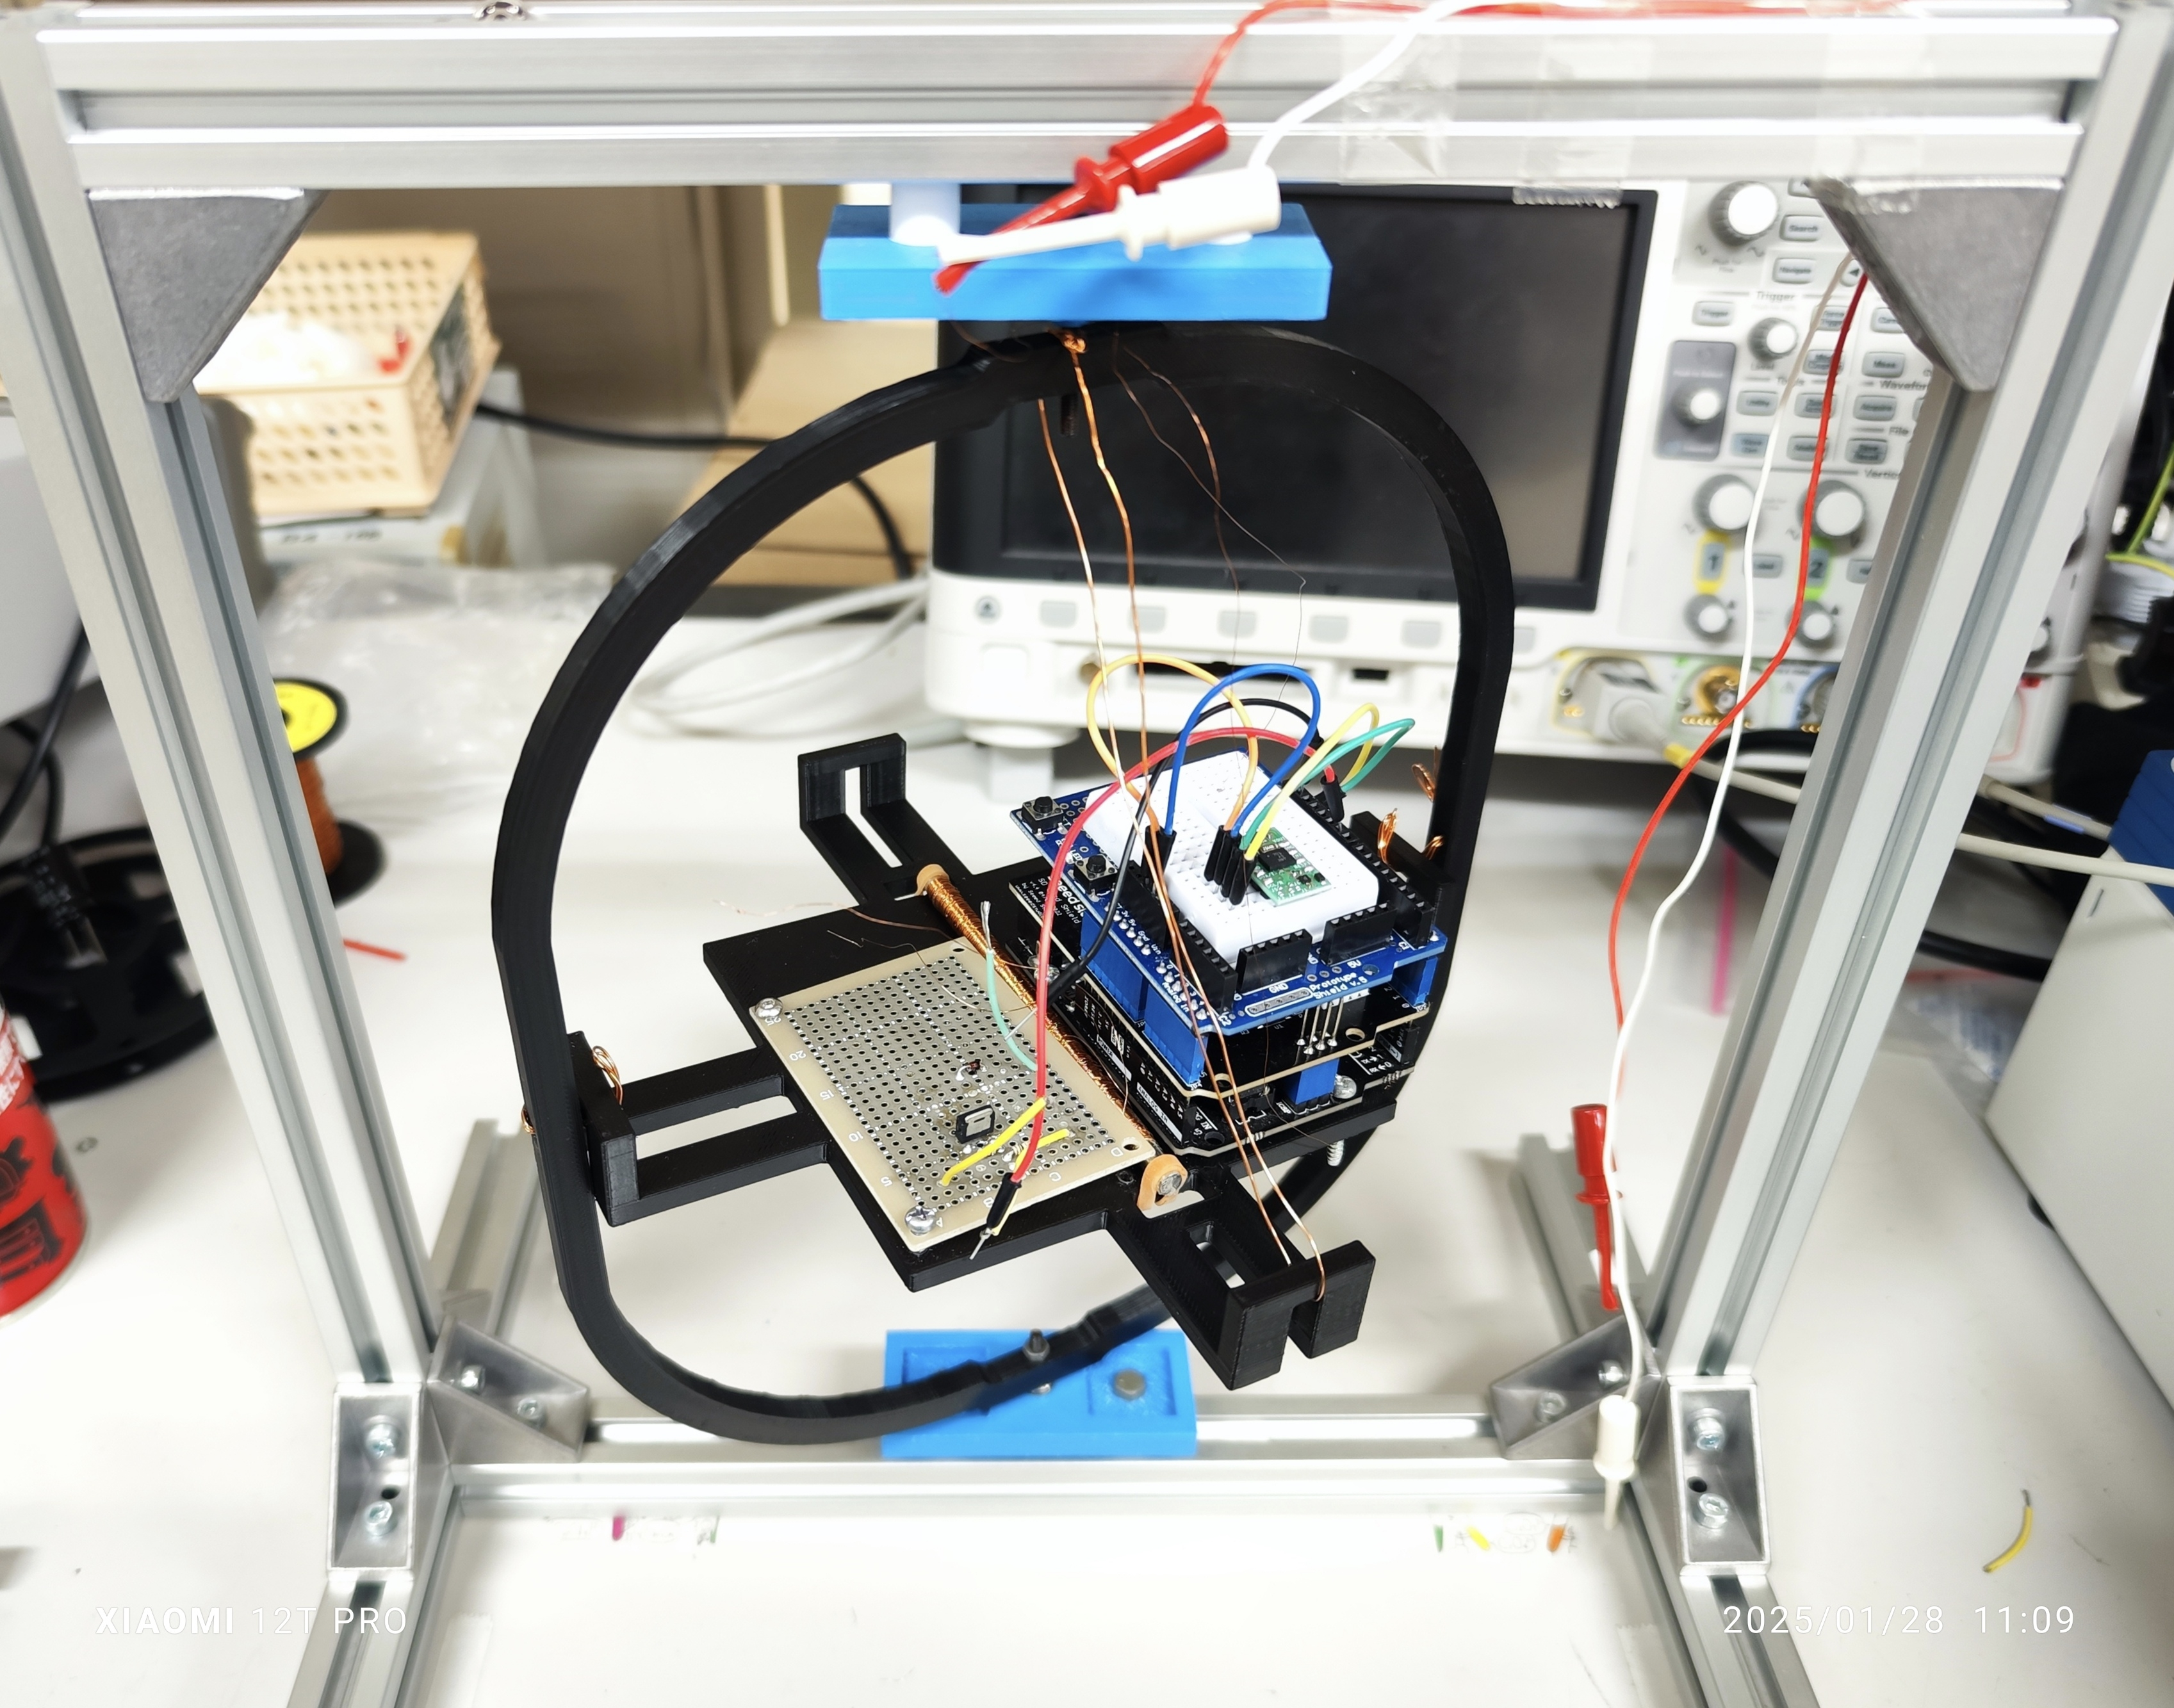
\includegraphics[scale=0.07]{./figure/実験装置.jpg}
		\caption{実験システムの外観}
		\label{fig:souti}
\end{figure}


\begin{figure}[H]
	\centering
		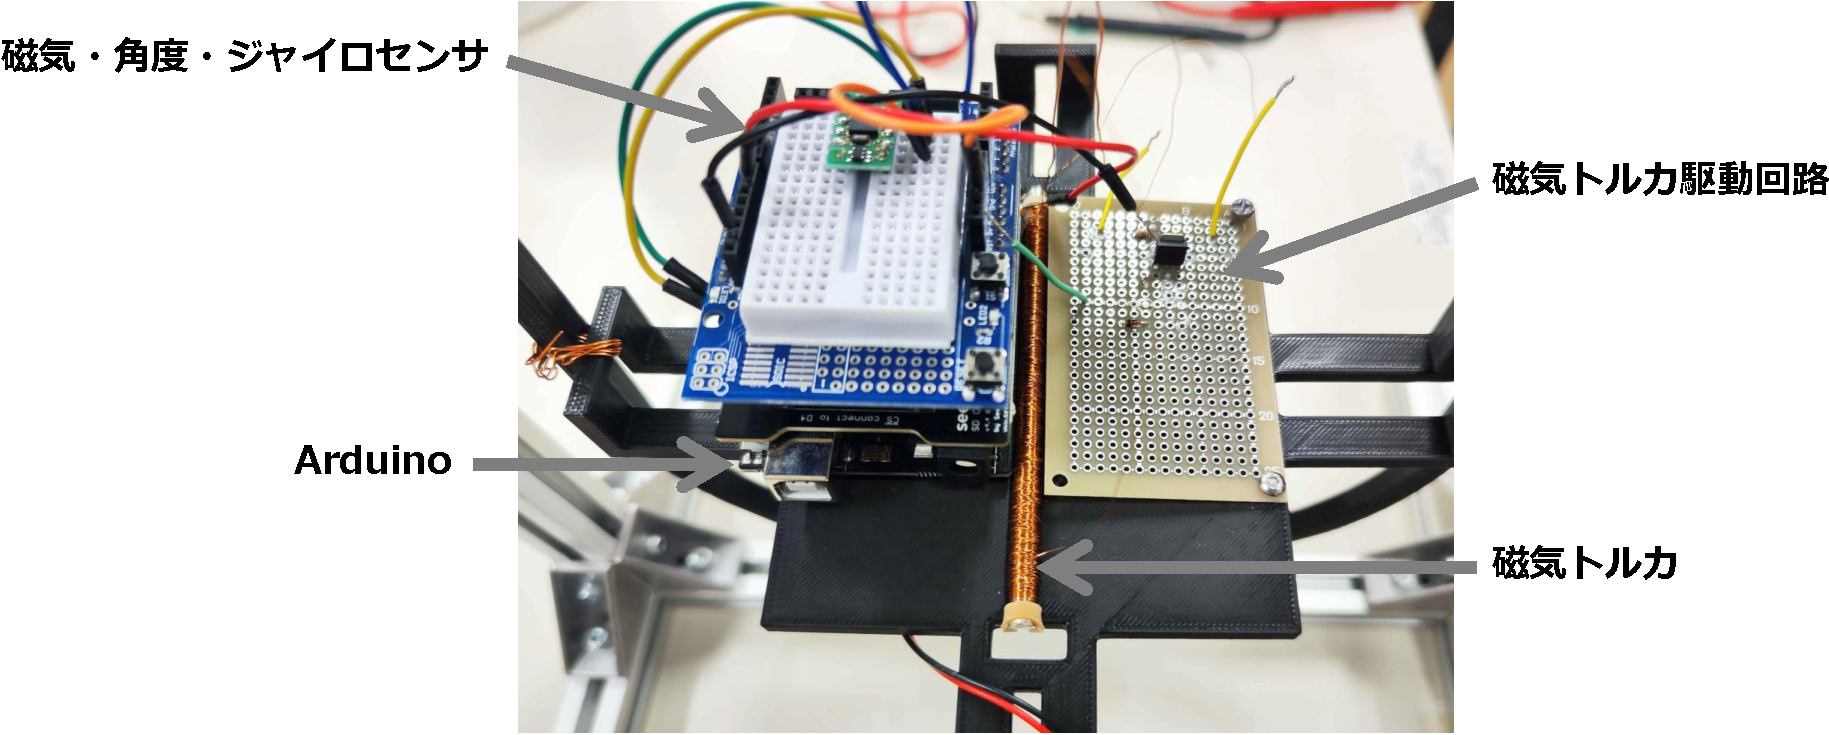
\includegraphics[scale=0.4]{./figure/実験システム.pdf}
		\caption{実験システムに搭載されている物品}
		\label{fig:system}
\end{figure}


\subsection{制御システムの設計}

 搭載するArduinoは,ELEGOO社製のArduino Uno R3を,開発環境にはArduino IDEを用いる.
姿勢角度,角速度および磁力の検出には,Bosch Sensortec社製のBNO055と,
Arduino IDEのライブラリ$"\mathrm{Adafruit\_Sensor.h}"$,$"\mathrm{Adafruit\_BNO055.h}"$
を用いる.また,姿勢角度,角速度および磁力の記録にはSDカードを用いており,
seeed studio社製のSD Card shield V4.0をArduinoに装着している.
Arduinoに書き込んだコードは,付録A.2に記す.
センサから取得した角度,角速度および磁気のデータを用いて,フィードバック制御を行う.
記録した角度・角速度のデータをCSVファイルに保存,それをPythonでグラフに描画し,姿勢角度の遷移を確認する.
実験システムの概要をブロック図にしたものを図\ref{fig:systemblock}に示す.

\begin{figure}[H]
	\centering
		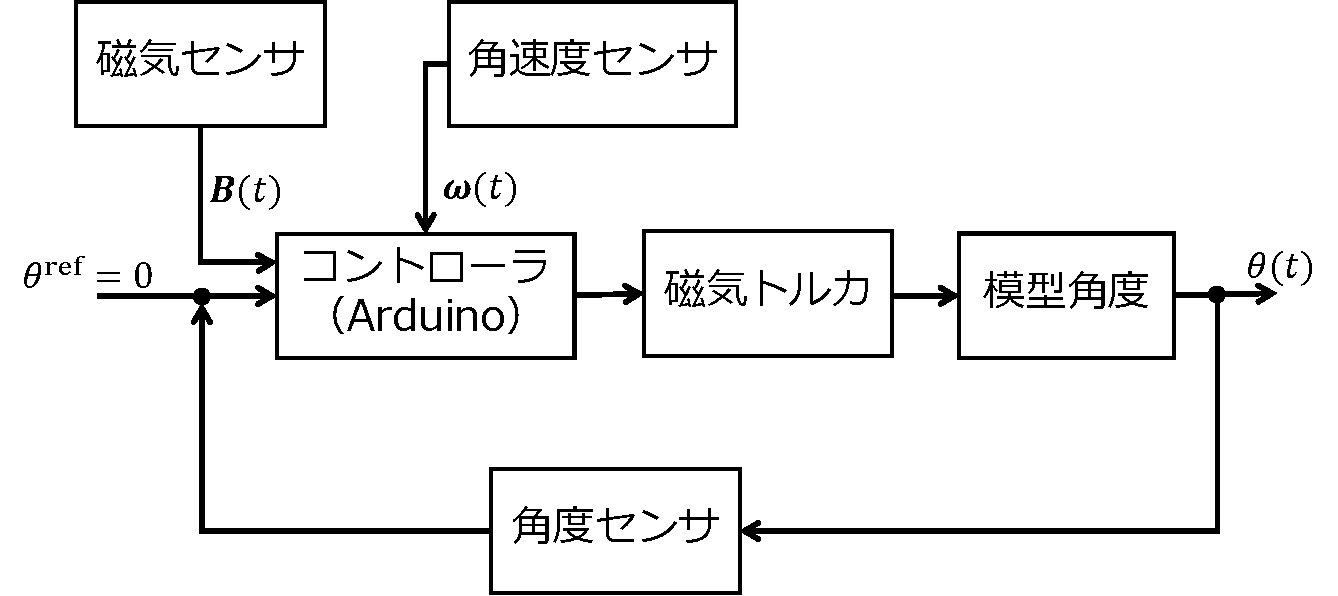
\includegraphics[scale=0.5]{./figure/block-crop.pdf}
		\caption{実験システムブロック図}
		\label{fig:systemblock}
\end{figure}

\begin{figure}[H]
	\centering
		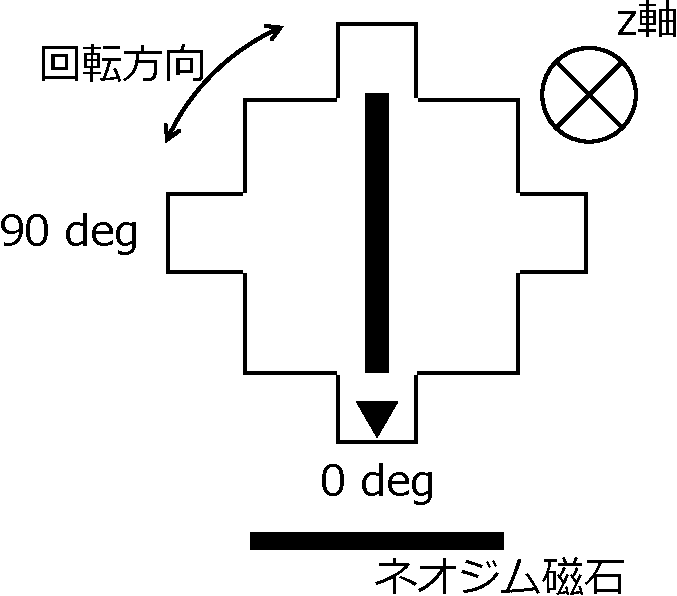
\includegraphics[scale=0.5]{./figure/system-crop.pdf}
		\caption{実験システム概略図}
		\label{fig:systemfig}
\end{figure}



\subsubsection{磁気トルカの作製}

 搭載した磁気トルカのパラメータを表\ref{table:torquer}に示す.
$\boldsymbol{E\text{-}B}$対応において,磁気トルカが発生させる磁気モーメントは,電流$I$,磁心の断面積$S$,断面の法線ベクトル$\boldsymbol{n}$を用いて,
\begin{equation}
	\boldsymbol{m}=IS\boldsymbol{n}
\end{equation}
と表される.また,地磁気を$\boldsymbol{B}_\mathrm{geo}$ [T] ,磁心の比透磁率を$\mu_r$とすると,磁気トルカがとらえる磁束密度は,
\begin{equation}
	\boldsymbol{B} = \mu_r\boldsymbol{B}_\mathrm{geo}
\end{equation}
となる.
そして,磁気トルカが発生させられるトルクは,磁気トルカの磁気モーメントと,磁気トルカがとらえる磁束密度を用いて,
\begin{equation}
	\boldsymbol{T = m \times B}
\end{equation}
と表される.
このことから,磁気トルカが生み出すトルクは比透磁率に比例していることがわかる.

 まず,芯材にステンレス鋼を用いて磁気トルカを作り,磁石を用いて反応性を確かめた.
しかし,ステンレス鋼の保磁力の高さのため,磁気トルカに電流を流していないときも磁力を持っており,
また比透磁率も低く,電流を流しているとき,いないときの差がなく磁力も低かった.
そこで比透磁率が高く,また保磁力が低い材料を探したところ,PCパーマロイ(Ni78\%)が条件を満足していたため,
ステンレス鋼を用いずPCパーマロイを用いて磁気トルカの作製を行った.
 芯材であるPCパーマロイの選定理由は,その透磁率の高さである.PCパーマロイは比透磁率が約180,000で,磁気トルカがとらえられる磁力が高くなる.
また,保磁力が低く,消磁しやすいため,必要な時だけトルクを発生させられる.
線材には,磁気トルカ作製によく用いられている銅線を,被膜は比較的安価なポリエステルとする.

\begin{table}[H]
	\centering
	\caption{磁気トルカのパラメータ}
	\label{table:torquer}
	\begin{tabular}{|c||c|}
		\hline
		コイル長さL [mm] & 100\\ \hline
		コイル直径D [mm] & 5\\ \hline
		巻き数n [-] & 983 \\ \hline
		比透磁率$\mu_r$ [-] & 約180,000 \\ \hline  
	\end{tabular}
\end{table}


%%%%%%%%%%%%%%%%%%%%%%%%%%%%%%%%%%%%%%%%%%%%%%%%%%%%%%
\subsection{磁気トルカの駆動回路}
%%%%%%%%%%%%%%%%%%%%%%%%%%%%%%%%%%%%%%%%%%%%%%%%%%%%%%
\subsubsection{駆動回路の設計}
 図\ref{fig:cirkit1}に,最初に構築した回路図を示す.
FETにはNchパワーMOSFET:2SK4017を用いている.ゲート閾値電圧は4~Vで,ArduinoのPWM出力は5~Vなので,FETを駆動させられる.
ArduinoからのPWM信号が2SK4017のゲートに入力され,PWMがONのとき,ドレイン-ソース間が導通し,磁気トルカに電流が流れる,といった仕組みとなっている.
この回路で,duty比50\%のPWM信号を入力した場合の,磁気トルカにかかる電圧を図\ref{fig:osiro1}に示す.なお,電圧のレンジは5~V/div~であり,磁気トルカの逆起電力が大きい.
そのため,FETがOFFのとき,磁気トルカに流れる電流が本来流すべき方向と逆方向に流れ,逆方向のトルクが発生することが
予測された.

\begin{figure}[H]
	\centering
		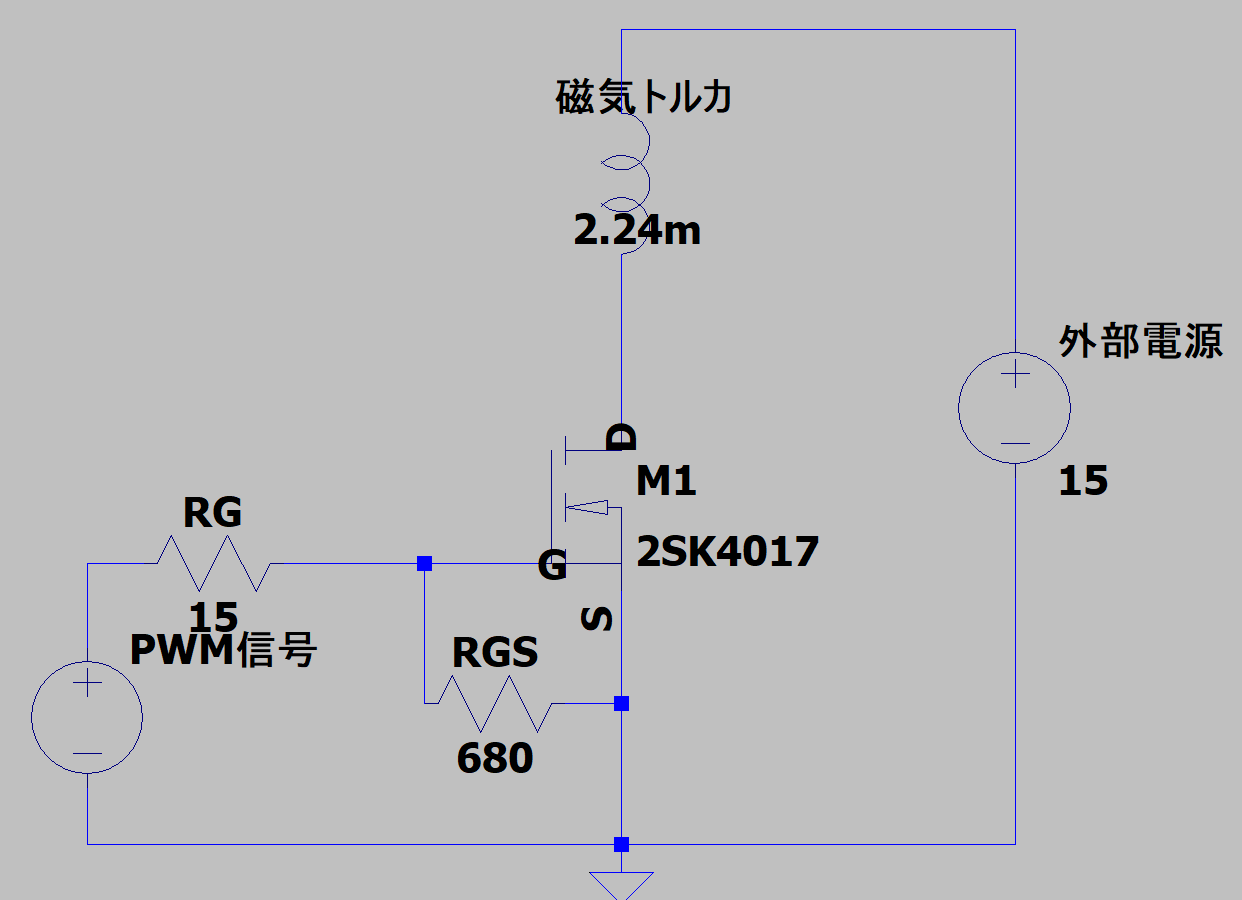
\includegraphics[scale=0.25]{./figure/回路図1.png}
		\caption{初期の磁気トルカの駆動回路}
		\label{fig:cirkit1}
\end{figure}

\begin{figure}[H]
	\centering
		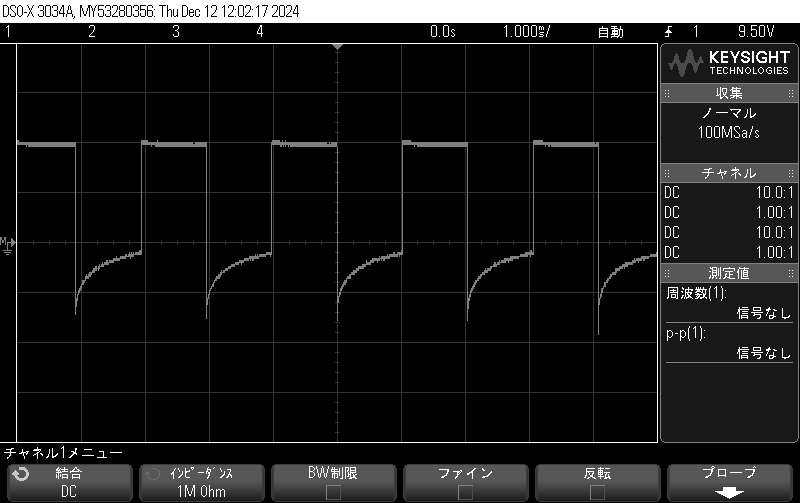
\includegraphics[scale=0.25]{./figure/scope_5.png}
		\caption{初期の駆動回路における磁気トルカに加わる電圧}
		\label{fig:osiro1}
\end{figure}


 そこで次に,磁気トルカと並列にダイオード(1N4148)を接続することで逆起電力を防止した.
作製した回路の回路図を図\ref{fig:cirkit}に示す.
具体的には,ON時に磁気トルカに蓄えられたエネルギーを,
ダイオードを通して閉回路となった磁気トルカの抵抗
により消費することにより,逆起電力を防ぐ.
この回路での磁気トルカにかかる電圧を図\ref{fig:osiro2}に示す.
このように,逆起電力を防ぐことができていることがわかる.


\begin{figure}[H]
	\centering
		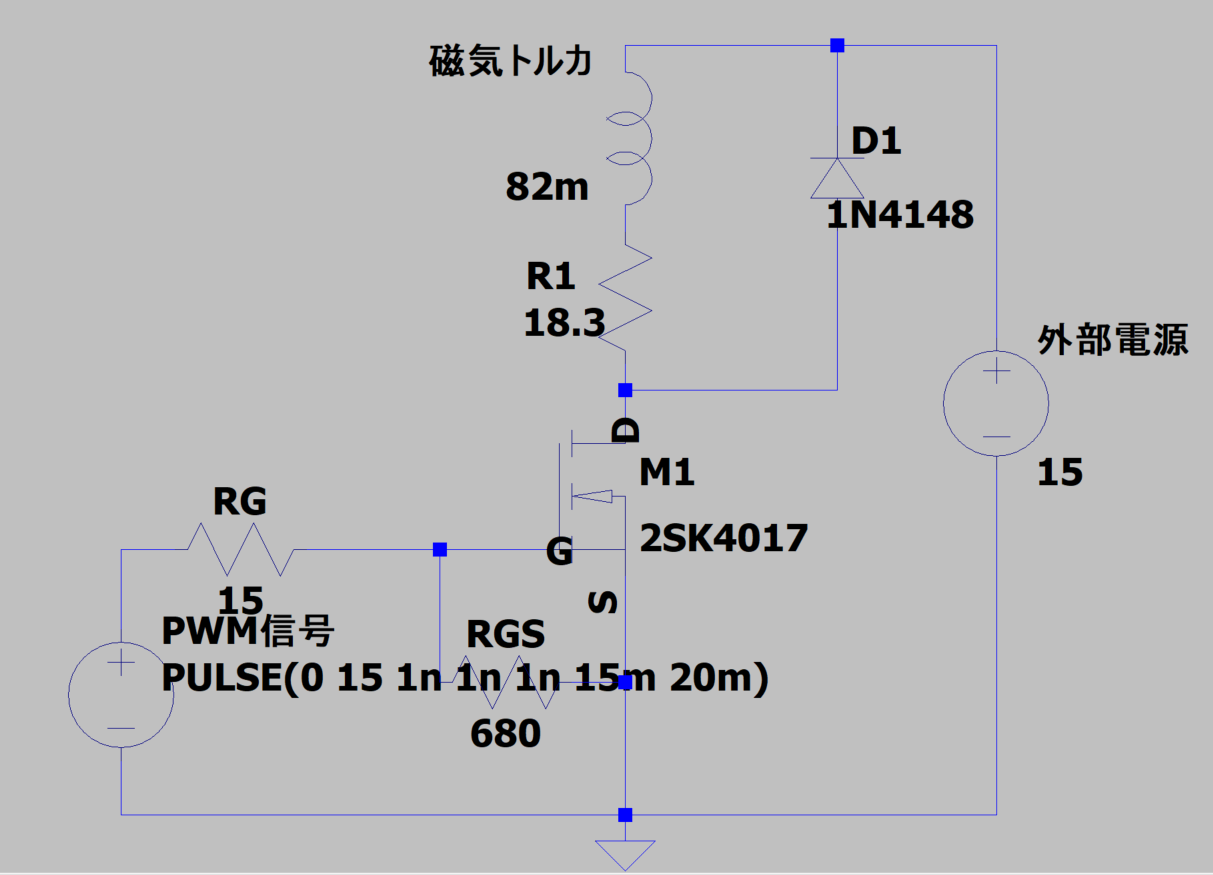
\includegraphics[scale=0.3]{./figure/駆動回路.png}
		\caption{改良した磁気トルカの駆動回路}
		\label{fig:cirkit}
\end{figure}

\begin{figure}[H]
	\centering
		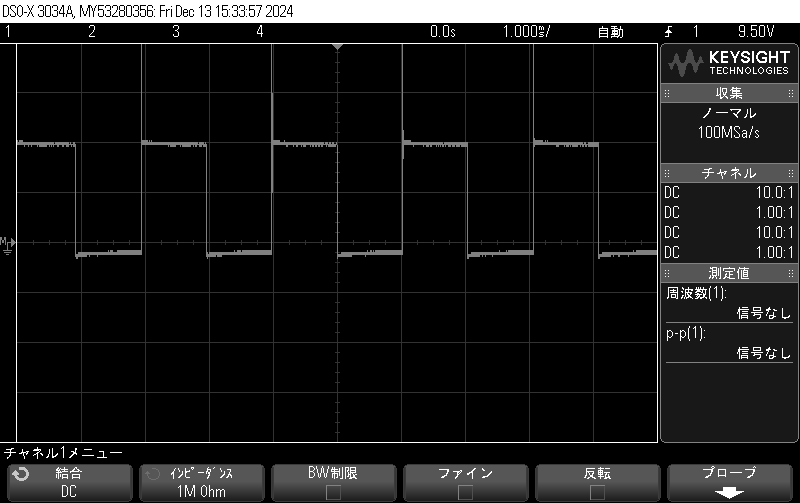
\includegraphics[scale=0.25]{./figure/scope_11.png}
		\caption{改良した駆動回路における磁気トルカに加わる電圧}
		\label{fig:osiro2}
\end{figure}

\subsubsection{磁気トルカの電流計算など}

 電流の制御をPWMで行うため,コイルの過渡特性を考慮して電流値の計算を行う必要がある.
一般的にコイルは,インダクタ成分のみでなく抵抗成分も含んでおり,低周波での等価回路は図\ref{fig:touka}のようになる.
よって,LR直列回路の過渡現象を考えればよい.
磁気トルカのインダクタンス,抵抗値は,表\ref{table:torquer2}に示す.
インダクタンスはLCRメータを,抵抗値はテスタを用いて測定した.LCRメータ,テスタは三和電気計器株式会社製のLCR700およびCD770を使用した.
外部電源の電圧値$E$ [V],抵抗成分$R_L [\Omega]$,インダクタンス$L$ [mH] から求められるFETがONのときの電流の過渡特性は,


\begin{equation}
	i(t) = \frac{E}{R_L}\left(1-e^{-\frac{R_L}{L}t}\right)
\end{equation}

で表される.また,FETがOFFとなったときの時刻を$t_1$ [s] とすると,その後の電流の過渡特性は,

\begin{equation}
	i(t) = \frac{E\left(1-e^{-\frac{R_L}{L}t_1}\right)}{R_L}e^{-\frac{R_L}{L}(t-t_1)}
\end{equation}

となる.さらに$t_2$ [s] 経過してFETがONになると,

\begin{equation}
	i(t) = \frac{E\left(1-e^{-\frac{R_L}{L}t_1}\right)e^{-\frac{R_L}{L}t_2}}{R_L}\left(1-e^{-\frac{R_L}{L}(t-t_1-t_2)}\right)
\end{equation}

で表される電流の推移をする.ここで,$D,t_1,t_2$の関係は,
\begin{equation}
	D = \frac{t_1}{t_1+t_2}
\end{equation}
で表される.また,$t_1,t_2$とDuty比$D$($0\leq D\leq1$),PWM周波数$f=490$~Hz~の関係は,
\begin{equation}
	t_1 = \frac{D}{f},t_2 = \frac{1-D}{f}
\end{equation}
となる.

\begin{table}[H]
	\centering
	\caption{磁気トルカの寄生成分}
	\label{table:torquer2}
	\begin{tabular}{|c||c|}
		\hline
		インダクタンス$L$ [mH] & 17.8 \\ \hline
		抵抗 $R_L$ [$\Omega $] & 18.3 \\ \hline 
	\end{tabular}
\end{table}

\begin{figure}[H]
	\centering
		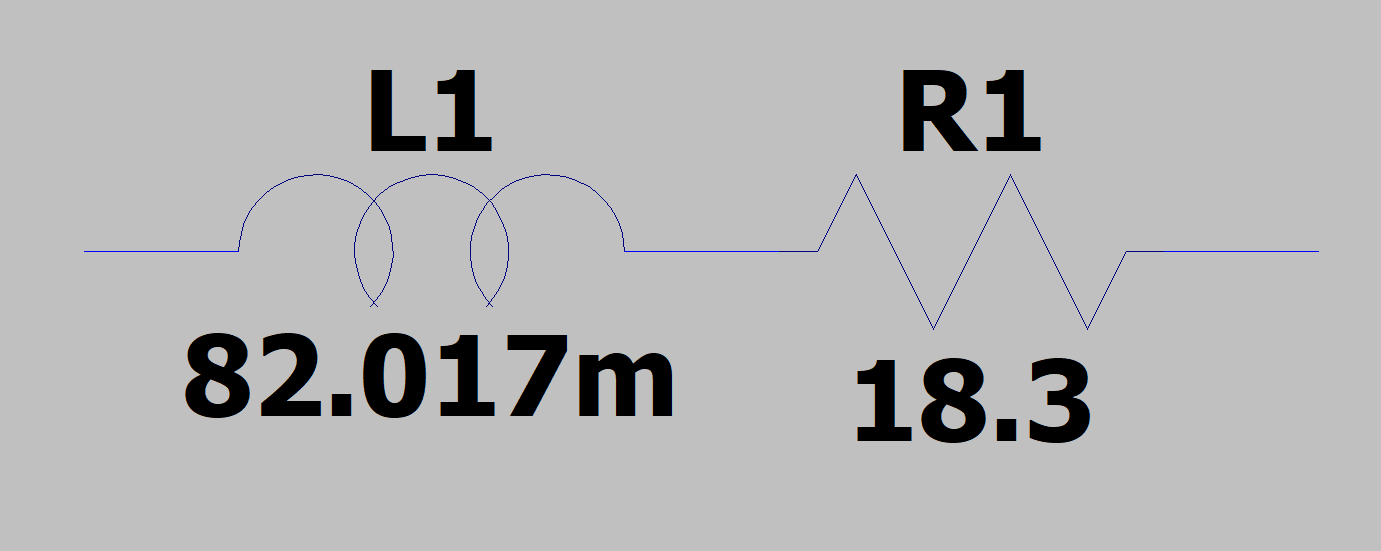
\includegraphics[scale=0.15]{./figure/touka.png}
		\caption{磁気トルカの等価回路}
		\label{fig:touka}
\end{figure}

この電流の推移を,図\ref{fig:cirkit}の回路を用いてduty比50\%でシミュレーションしたグラフを図\ref{fig:current50}に示す.
このように,磁気トルカに電圧$E$~[V]~を印加したときの電流を$I_\mathrm{max}~[\mathrm{A}]~$とすると,duty比$D$のPWM信号で磁気トルカを駆動させたとき,
およその電流を$I(D)=I_\mathrm{max}D~[\mathrm{A}]~$で近似できる. 
そのため電流$I$を流したいときは,
\begin{equation}
	D=\frac{I}{I_\mathrm{max}}
\end{equation}
でDuty比を決定する.なお,$I_\mathrm{max}=\frac{E}{R_L}=\frac{15}{18.3}\approx0.82~\mathrm{mA}~$である.


\begin{figure}[H]
	\centering
		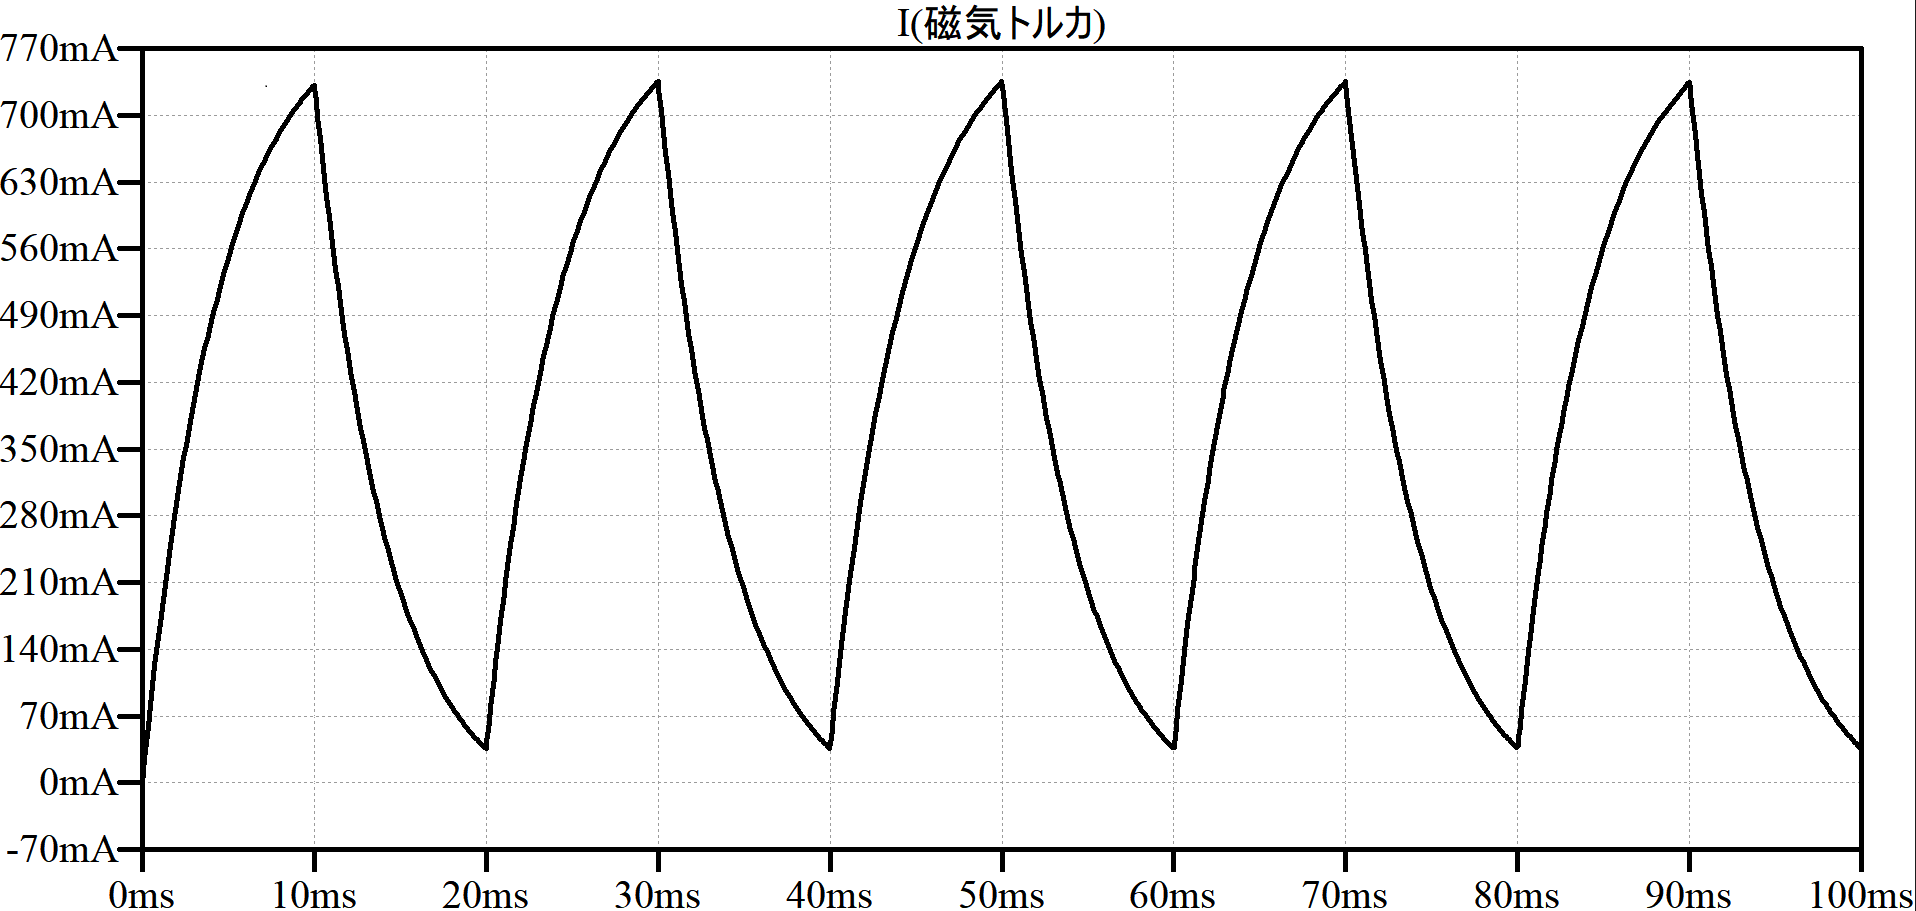
\includegraphics[scale=0.25]{./figure/50current.png}
		\caption{磁気トルカに流れる電流}
		\label{fig:current50}
\end{figure}

\subsection{磁束密度の測定結果}

 磁気トルカに電圧を印加し,発生する磁束密度をシロ産業社製のハンディガウスメータMG-501で測定した.
その結果を図\ref{fig:magnetic_flux_density}に示す.
今回磁気トルカ駆動用回路に用いた外部電源の電圧は15~V~であるが,図\ref{fig:magnetic_flux_density}の結果から,
電圧に対する磁束密度の線形性を維持できているのは5~V~近傍までである.
今回用いたPWM制御のDuty比で表すと約33\%となる.

\begin{figure}[H]
	\centering
		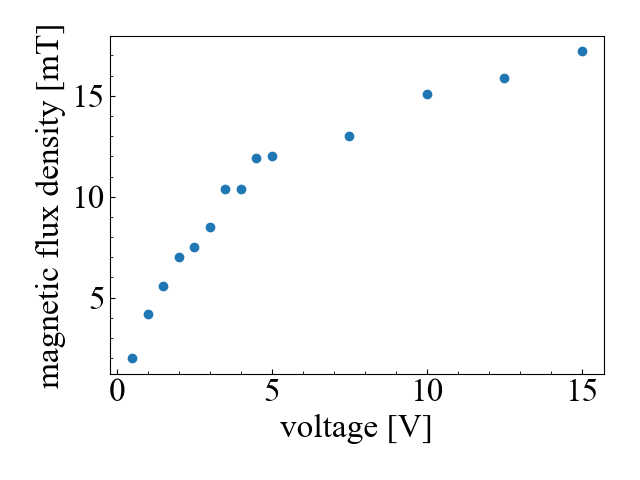
\includegraphics[scale=0.45]{./figure/figure.png}
		\caption{電圧値に対する磁気トルカの磁束密度}
		\label{fig:magnetic_flux_density}
\end{figure}